
Between 1997 and 2005, the Laboratoire G\'enie de Production of the National Engineering School of Tarbes developed an Explicit Finite Elements Code for the numerical simulation of the behavior of mechanical structures subjected to impacts in large thermomechanical deformations: the DynELA FEM code. This academic FEM code has been used as a support for different PhD thesis and several scientific publications \cite{Pantale:2002,Pantale:2004,Menanteau:2006,Nistor:2007,Nistor:2008} among which one was focused on the parallelization of the DynELA FEM code using the OpenMP library \cite{Pantale:2005}. The purpose of this paper is to present the steps that have been made necessary in order to allow the reproduction of the results presented in the article \cite{Pantale:2005} using the original 2005 version of the DynELA code.

\section{Historical context}

During my thesis work (1992-95), the reflections carried out with my thesis supervisor led me to propose a new research theme focused on the numerical development of a FEM code in large deformations: the DynELA FEM code. Traditionally, FEM codes are programmed using procedural programming languages such as Fortran or C. In the spirit of procedural languages, adding new features to already very long programs requires programmers to work with a complexity that increases exponentially with the initial size of the code. Object-Oriented Design and Programming (OOP) methods are best suited to large-scale developments. The abstraction allowed by OOP allows the developer to better organize the architecture of the program and to anticipate future developments. From a programming language point of view, if the preferred current general standard is to use C++, other languages can be used for the development of numerical applications. Concerning our work, the C++ language was used for the numerical implementation of the FEM code DynELA. The main characteristics of this code are: an explicit integration scheme and a formulation in large deformations, an Object-Oriented approach for the numerical implementation in C++ and a totally open code architecture based on own developments and use of open-source libraries.

This work was mainly motivated by the fact that the development of a FEM code allows a very important personal intellectual enrichment. The numerical developments allow to deepen the knowledge in the field of mechanics in large deformations since one is obliged to master the theory in order to be able to implement it numerically. It is a phase of consolidation of knowledge directly through experience, certainly more delicate, but much more thorough.

\subsection{Architecture of the FEM code}

In a finite element code development process, the preliminary phase consists in defining a set of basic libraries for data management (in the form of lists, stacks, ...) as well as the various mathematical libraries adapted to the modeling cases encountered. The choice retained in this work was to develop entirely the set of basic libraries and to encapsulate a part of the Lapack \cite{Lapack:1999} mathematical library in order to develop new matrix and tensor classes, because no mathematical library was available for this purpose. For example, classical mathematics does not propose the notion of 4th-order tensor. The FEM code DynELA is composed of a set of separate libraries and executable files that have each of the particular tasks. A simplified list of these libraries is given below:
\begin{itemize}
\item basicTools: basic library which contains the basic classes of the DynELA application.
\item linearAlgebra: algebraic calculation library. It defines in particular the notions of vectors, matrices, tensors and mathematical functions. This one encapsulates part of the Lapack and Blas libraries.
\item interpretor: library that defines the interpreted command language of DynELA. It was one of the strong points of the original software.
\item femLibrary : finite element computation library (it is the heart of the finite element solver).
\end{itemize}
From these various libraries, we created a set of executable programs that correspond to the various modules of the FEM code: the finite element solver, the graphics post-processor, the curve analysis program, the language generator, etc...

\subsection{Specificities of the DynELA FEM code}
In terms of size of development, even if this notion is not very scientific since you can artificially increase the size of a code (by duplicating pieces of source unnecessary for example), one can globally estimate the number of C++ lines of code for the different modules as follows:
\begin{itemize}
\item Command interpreter: 10,000 lines of C++ code, Flex and Bison \cite{Levine:2009}
\item Graphics post-processor: 20,000 lines of C++ code
\item Finite element solver: 80,000 lines of C++ code.
\end{itemize}

\subsubsection{Command interpreter}
One of the major points in the development of a FEM code lies in the way the user specifies the data of a model. Several alternatives are possible. Some softwares privilege the use of a graphical interface allowing to build step by step the numerical model, others use a command file that the user edits externally. In the approach adopted, an advanced command language has been retained as the main means of defining a numerical model. 

The trend at the time of this work was towards the development of command languages for driving simulation codes to replace the command files inherited from the punched card era that were still found in many numerical codes. Concerning the DynELA FEM code, the choice fell on the development of a specific lexical and grammatical parser developed using standard Flex and Bison tools. Generally speaking, this command file has a syntax close to the C++ language and allows the manipulation of object-oriented data, the writing of tests and loops. 
 
\subsubsection{Graphics post-processor}

The evaluation of the numerical results is carried out by means of a graphical post-processor specially developed for the DynELA FEM code. The 3D graphical part uses OpenGL formalism, and the construction of the interface is carried out using the QT graphical library. Concerning these two libraries, the porting of the post-processor to the new architecture did not pose any problems concerning the OpenGL library, on the other hand, concerning the QT library, the initial version was based on QT-3, but the porting to QT-4 was carried out between 2005 and 2010 for the continuity of the work related to the various PhD thesis in progress over this period. The version used in this work is therefore the one developed in 2010.

\subsubsection{Finite element solver}

The finite element solver used in this work is version v.1.0 developed in the laboratory between 1996 and 2005, the date of production of the referenced paper. The finite element solver has subsequently evolved after 2005 and up to 2010, but since this version is subsequent to the publication of the referenced paper, it will not be used for this work. Moreover, in 2005, there were 2 versions of the FEM code: a classical version (the one that has continued to evolve) and a parallel version (not modified afterwards), and it is the latter that will be used afterwards.

\subsection{Computational context of the original publication}
Concerning the developments carried out within the framework of the publication selected for this work \cite{Pantale:2005}, the choice of the physical architecture was a Compaq Proliant 8000 SMP machine running under Linux Redhat 8.0 environment. This machine, which is illustrated in Figure \ref{proliant} was equipped with 8 Intel Xeon PIII 550/2Mb processors around a 5Gb shared main memory. 
\begin{figure}[h] 
  \centering
  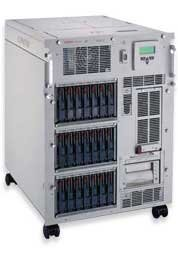
\includegraphics[width=0.3\textwidth]{./8000_photo.jpg}
  \caption{The Compaq Proliant 8000 SMP machine}
  \label{proliant}
\end{figure}
The compilation of the source code was performed by the Intel Cpp 7.1 compiler without optimization parameters in order to be able to compare the different parallelization techniques without any influence of the compiler. The OpenMP standard has been chosen for code parallelization.

\section{Retrieval of the software}

Between 2010 and 2018, different orientations of the research activities put aside the intensive development phase of this Finite Element code, nevertheless, since september 2018, a new version in C++ and Python has started in order to refurbish this numerical tool and to allow new developments. This modified version is based on the latest version (the 2010 version) for which many modifications have been made, among which the main ones are:
\begin{itemize}
\item The pure and simple abandonment of the graphical pre- and post-processor part (based on the QT and OpenGL libraries), replaced for the exploitation part of the results by a class for writing the results in VTK format allowing the use of the paraview graphical post-processor.
\item The replacement of the original command language based on the use of Flex and Bison tools by a Python interpreter via the SWIG tool.
\end{itemize}

\subsection{Finding the source code}

First of all, finding the complete source code of the version used for publication was not an easy task. Indeed, the different versions were developed and archived on various digital supports (floppy disks, CDROM, floppy ZIP, ...), the incremental numbering was not always respected, and by bad luck, the Proliant server which contained the version used for the production of the scientific publication was scrapped without saving the sources of the latest version of the code (or else, the backup has been purely lost since). It was nevertheless possible to rebuild a version close to the final version based on the modification history starting from a classical 1.0 version and modifying the files involved in the implementation of the parallel computing that had been saved by chance. In fact, only the files modified between the parallel version and the classic version could be found. The first point that emerges from this analysis and the difficulties related to the recovery of old source code concerns the need to improve the procedures for archiving the source code of the softwares developped in our laboratory.

As presented above, the DynELA code is composed of several thousand C++ lines of code located in an organized tree structure, which more or less facilitated the compilation procedure. The compilation of the various modules must be chained directory by directory, a library being compiled in each main sub-directory. The number of dependencies and the complexity of the code tree made it necessary to use a tool not used at the time of the initial development, the CMake \cite{CMake} utility for the generation of different Makefiles in the source directories. At the time of development, the Makefiles were handwritten, and the compilation of the sources was done directly in the source directories themselves (which is absolutely not a good thing to do), we had a mixture of C++ sources, headers and compiled objects in the same directory.

So the first step was to reorganize the sources on one side, a Build tree in a separate directory and to create a set of compilation directives for the CMake utility. Of course, we also had to take into account the requested dependencies concerning external libraries: Flex and Bison \cite{Levine:2009} mainly, but this phase does not pose any problem as these libraries are standard on Linux, and one just have to install them using an appropriate ubuntu package. The old Makefiles contained all the needed information concerning the requested libraries.

\section{Compilation, update of the code and benchmarks}

Since the machine used at the time of the publication of the proposed paper (in 2005) has been scrapped since then, the implementation of this work was done on a Dell R730 server equipped with 24 Intel Xeon E5-2650 2.20GHz cores and 96Gb of RAM. This server runs under Ubuntu Bionic 18.04.4 LTS with a 4.15.0-76 kernel. 

The hardware configuration is therefore clearly different from the one used in the original article, so we can expect that, if the Finite Element code runs correctly and gives numerical results in agreement with those obtained in the original paper, as it will be presented further, the performance and the behavior with respect to code parallelization will differ due to the change in processor architecture, memory and especially the evolution of the Operating System.

\subsection{Compilation of the code}

The compilation of the DynELA code is done using the standard compiler on Ubuntu 18.04.4 LTS: the c++ 7.4.0. Flex and Bison versions are 2.6.4 and 3.0.4 respectively. The parallelization is done using the -fopenmp compiler option and the OpenMP parallelization libraries is provided by the gcc-7 library.

During the compilation of the code, a number of warning messages are generated (mainly concerning functions not explicitly defined at compile time), which did not exist at the time of the initial work, however these have been ignored and do not seem to be detrimental to the proper compilation of the source code or its execution. The compilation part of the Lapack and Blas mathematical libraries is done without any problem (note that these libraries have been translated from Fortran by the f2c utility and are part of the CLAPACK and CBLAS packages). In the modern version of the DynELA code, this part of the source code has been removed and replaced by the use of the Lapacke and Blas libraries.

\subsection{Adaptations of the code}

The main change made to the Finite Element code concerns the subroutine execution time measurement class used to know precisely the times spent in the various parts of the program. In fact, during the first executions, the times reported by the original class were outliers. It was therefore decided to simply replace the measurement made by this old class by the class for measuring execution times taken from the new version of the DynELA code, hopefully there were compatible one to the other one. It is this new class which was used thereafter to measure the speedups of the code according to the number of CPUs used. The measurement points in the code were thus modified in order to take into account this new means of measuring CPU times.

\subsection{Comparison of results vs. the original paper}

\subsubsection{Comparison of numerical results}\label{Ptensile}

After the compilation phase, the first operation was to re-launch the simulations made during the preparation of the initial publication and to compare the results obtained with those obtained in 2005. In order to illustrate this step, Figure \ref{strain} shows the results obtained for the numerical simulation of a dynamic tensile test with on the left side the initial mesh, and on the right side the final the deformed plastic strain contourplot, in a similar way to Figure 9, page 370 of the initial paper \cite{Pantale:2005}. 
\begin{figure}[h!] 
  \centering
  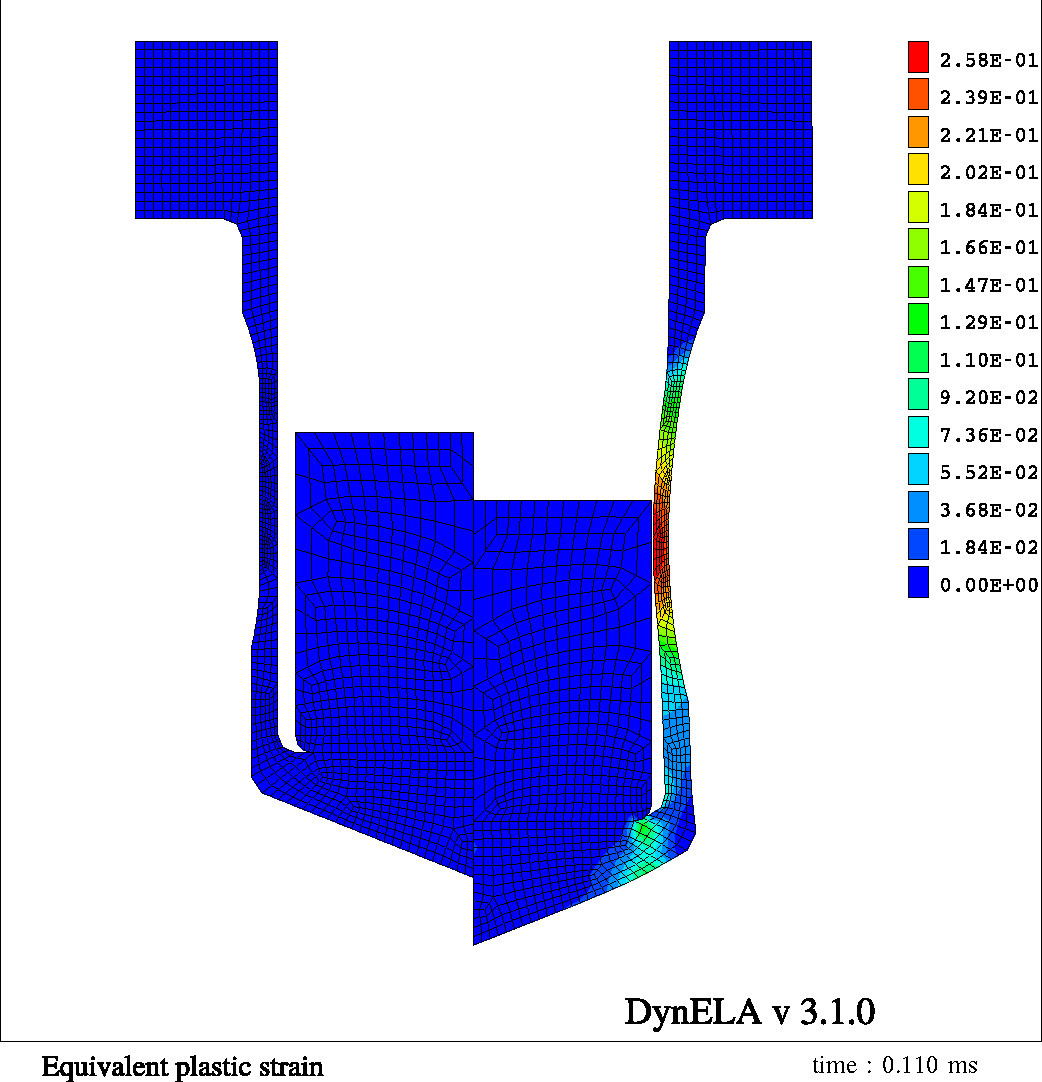
\includegraphics[width=0.6\textwidth]{./strain.pdf}
  \caption{Dynamic traction: initial mesh and equivalent plastic strain contour}
  \label{strain}
\end{figure}
The original figure has not been reproduced here, but one can notice the very good agreement between the two simulations allowing to validate the global behaviour of the FEM code. Other comparisons have been made to validate that the code does indeed give the same numerical results as in its 2005 version, but are not reported in this article. The good agreement between the two versions makes it possible to validate the correct behavior of the code between its two deployments 15 years apart. No crashes of the computation code, segmentation fault type problems, or other problems that could suggest an instability of the code structure have been noted. Only abrupt stoppages due to data errors were encountered, but they are similar to those obtained in the preliminary version (so the errors also are reproducible).

\subsubsection{Internal forces computation parallelization}

The main subject of the original publication produced in 2005 concerns the parallelization of the DynELA code and \textbf{the influence of the strategies on the Speedup}. In a second step, we will therefore relaunch the numerical simulation of the different code parallelization strategies and try to reproduce the results obtained in 2005. To do so, and in order not to present the whole tests, we will focus on the parallelization of the part concerning the computation of the internal forces (presented in paragraph 4.3 page 367 of \cite{Pantale:2005}) mainly for the Taylor test with a mesh consisting of 6500 finite elements (as presented in paragraph 4.2 page 367 of \cite{Pantale:2005}). In the original paper, 4 parallelization methods were studied, even though the DynELA code has in its original version 8 different methods available. Simulations have been redone with these 8 parallelization methods, and the results in terms of speedup for the 4 corresponding to the 2005 paper are reported in Figure \ref{speedup}.
\begin{figure}[h!] 
  \centering
  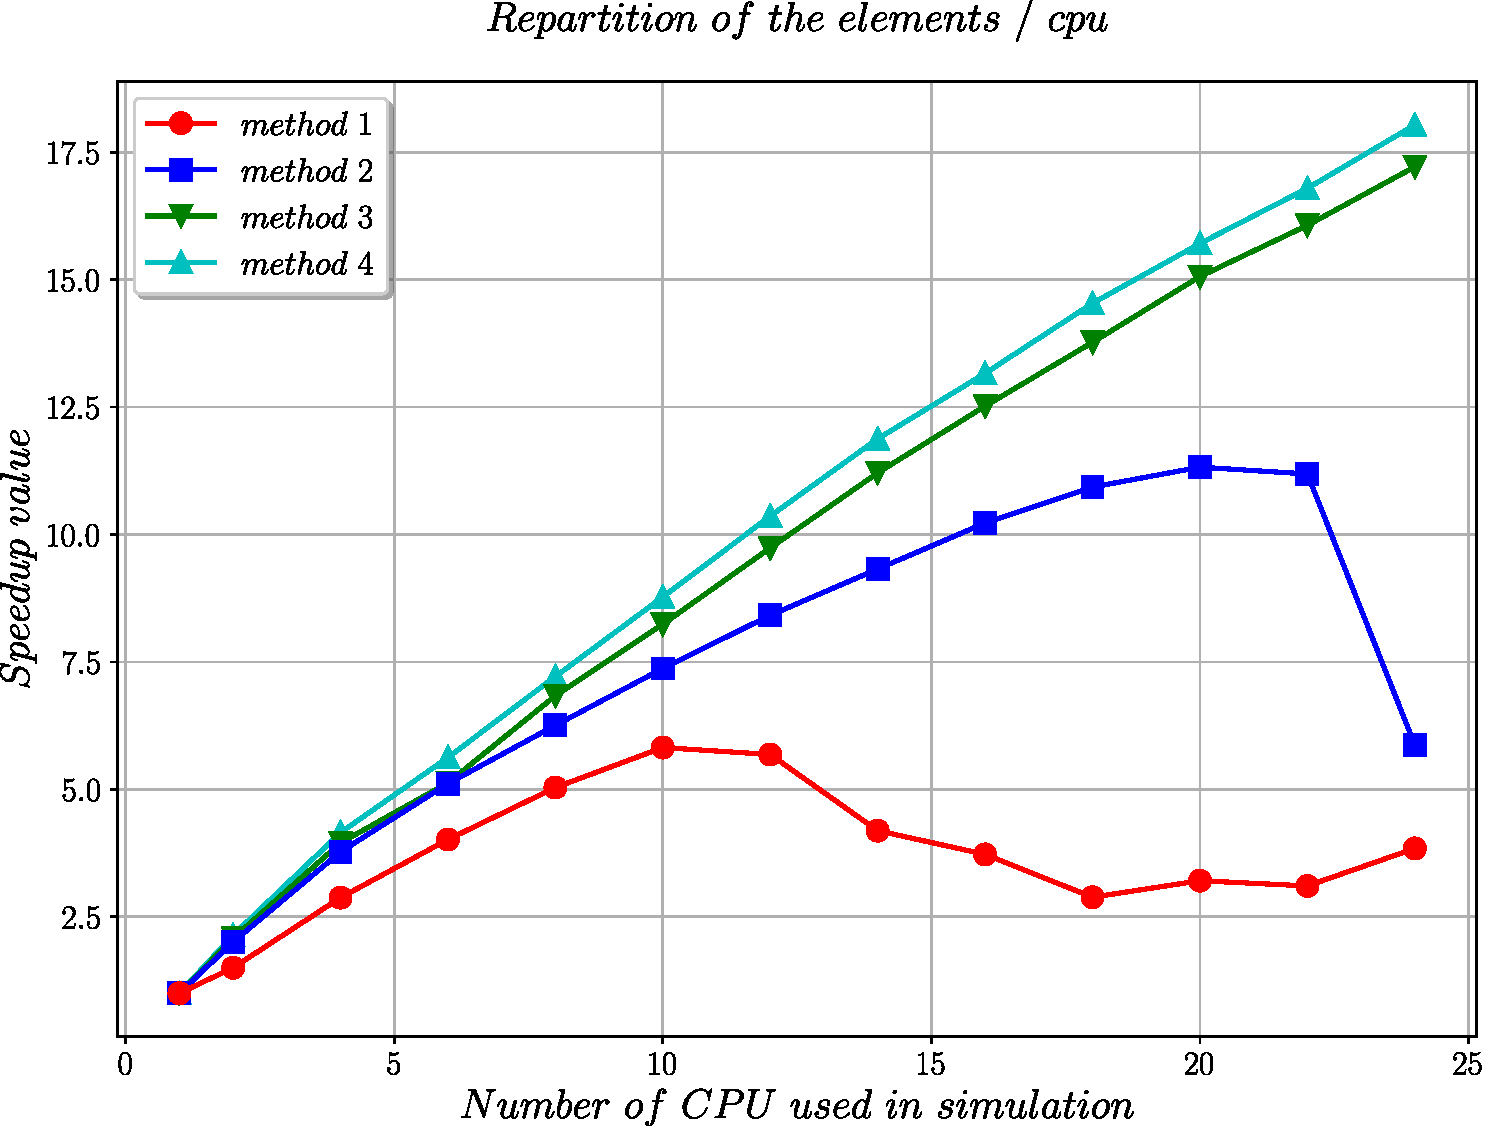
\includegraphics[width=0.75\textwidth]{./speedup.pdf}
  \caption{Speedup of the $\protect\overrightarrow{F^{int}}$ computation for various implementations}
  \label{speedup}
\end{figure}
The comparison of the results of Figure \ref{speedup} and of Figure 7 page 369 of \cite{Pantale:2005} shows a good accordance of the numerical results even if the architectures used in the two cases differ significantly. We can thus notice that, since the current server has 24 CPUs, we were able to extend the analysis beyond the 8 CPUs originally used. The speedups obtained in the current version are globally lower, but this can be explained by:
\begin{itemize}
\item the fact that the OS used is much more multitasking than the one used in 2005, which means that the machine has a different workload,
\item the hardware architecture also differs, the working disks are now on another server, and we use an NFS protocol that can have an impact on code parallelization performance,
\item the numerical model is identical to the one used in 2005, but in order to have a significant gain on a large number of CPUs (range beyond 8), the size of the model would have to be larger in order to ensure that each CPU can handle a sufficient number of elements to justify the use of parallelization (roughly speaking, fork and join times become non-negligible when the load/cpu decreases). But this would have changed with regard to the original test published.
\end{itemize}
Nevertheless, and despite these differences, we can notice that the current version reproduces the same trends as the simulation done in 2005 and that method 4 provides an ever increasing speedup as a function of the number of CPUs while method 1 shows its limits very quickly. The same conclusions can therefore be drawn concerning the parallelization of the code as those obtained in the article \cite{Pantale:2005}, which shows the reproducibility of the results.

\subsubsection{The load balancing algorithm}

Finally, in this last part, we will compare the results obtained by the load balancing algorithm in the computation of the internal force vector. This algorithm seeks during the calculation to minimize the waiting time of the different CPUs in the parallel internal force vector evaluation phase by dynamically changing the number of elements allocated to each CPU during the computation. The original results are presented in paragraph 5 on page 371 of the article \cite{Pantale:2005}.

For this simulation the test case of the tensile test presented in paragraph \ref{Ptensile} is used again. Thus, Figure \ref{spacethreads} shows the spatial distribution of the elements for the numerical simulation of the tensile test on 4 CPUs over time, respectively at the beginning of the simulation (left part of the figure), at 50\% of the calculation (middle part of the figure) and at the end of the calculation (right part of the figure). Obviously, the comparison with Figure 11, page 372 of the article \cite{Pantale:2005} shows differences iconcerning the localization of the elements with respect to the different processors, as well as Figure \ref{timethreads}, to be compared with Figure 12 page 373 of the article \cite{Pantale:2005}. Nevertheless, the same global remarks can be made about the load balancing algorithm used in the DynELA code. It is therefore clear that the number of elements processed by each CPU evolves over time in order to balance the loads of each CPU during the calculation.

In conclusion of this comparative part, we can say that even if the local results in terms of parallelization gain, localization of the elements with respect to the different processors, are more or less different, the global behavior of the DynELA code is satisfactory. The results of the numerical simulations are in agreement with the results obtained in the simulations carried out in 2005.

\begin{figure}[h!] 
  \centering
  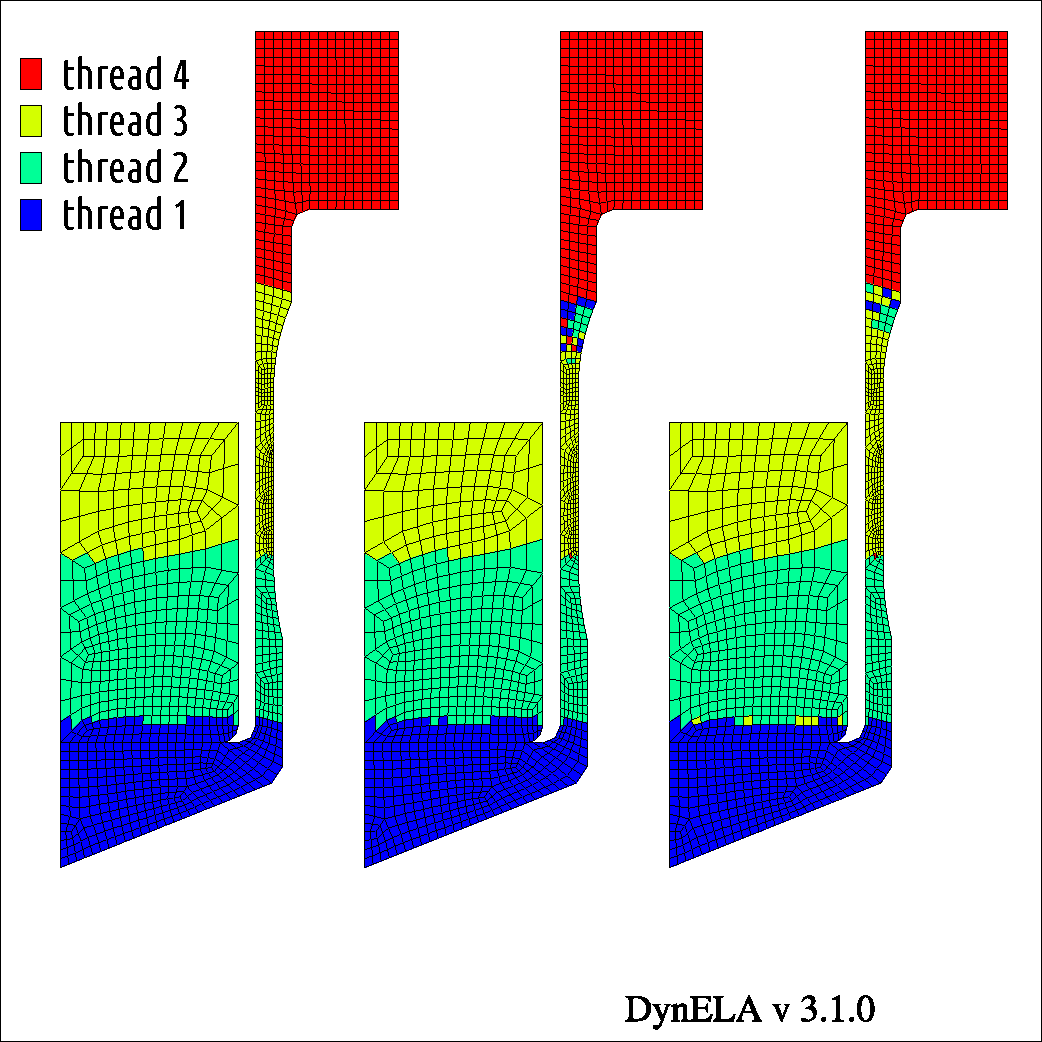
\includegraphics[width=0.6\textwidth]{./spacethreads.pdf}
  \caption{Spatial distribution of the elements during computation}
  \label{spacethreads}
\end{figure}

\begin{figure}[h!] 
  \centering
  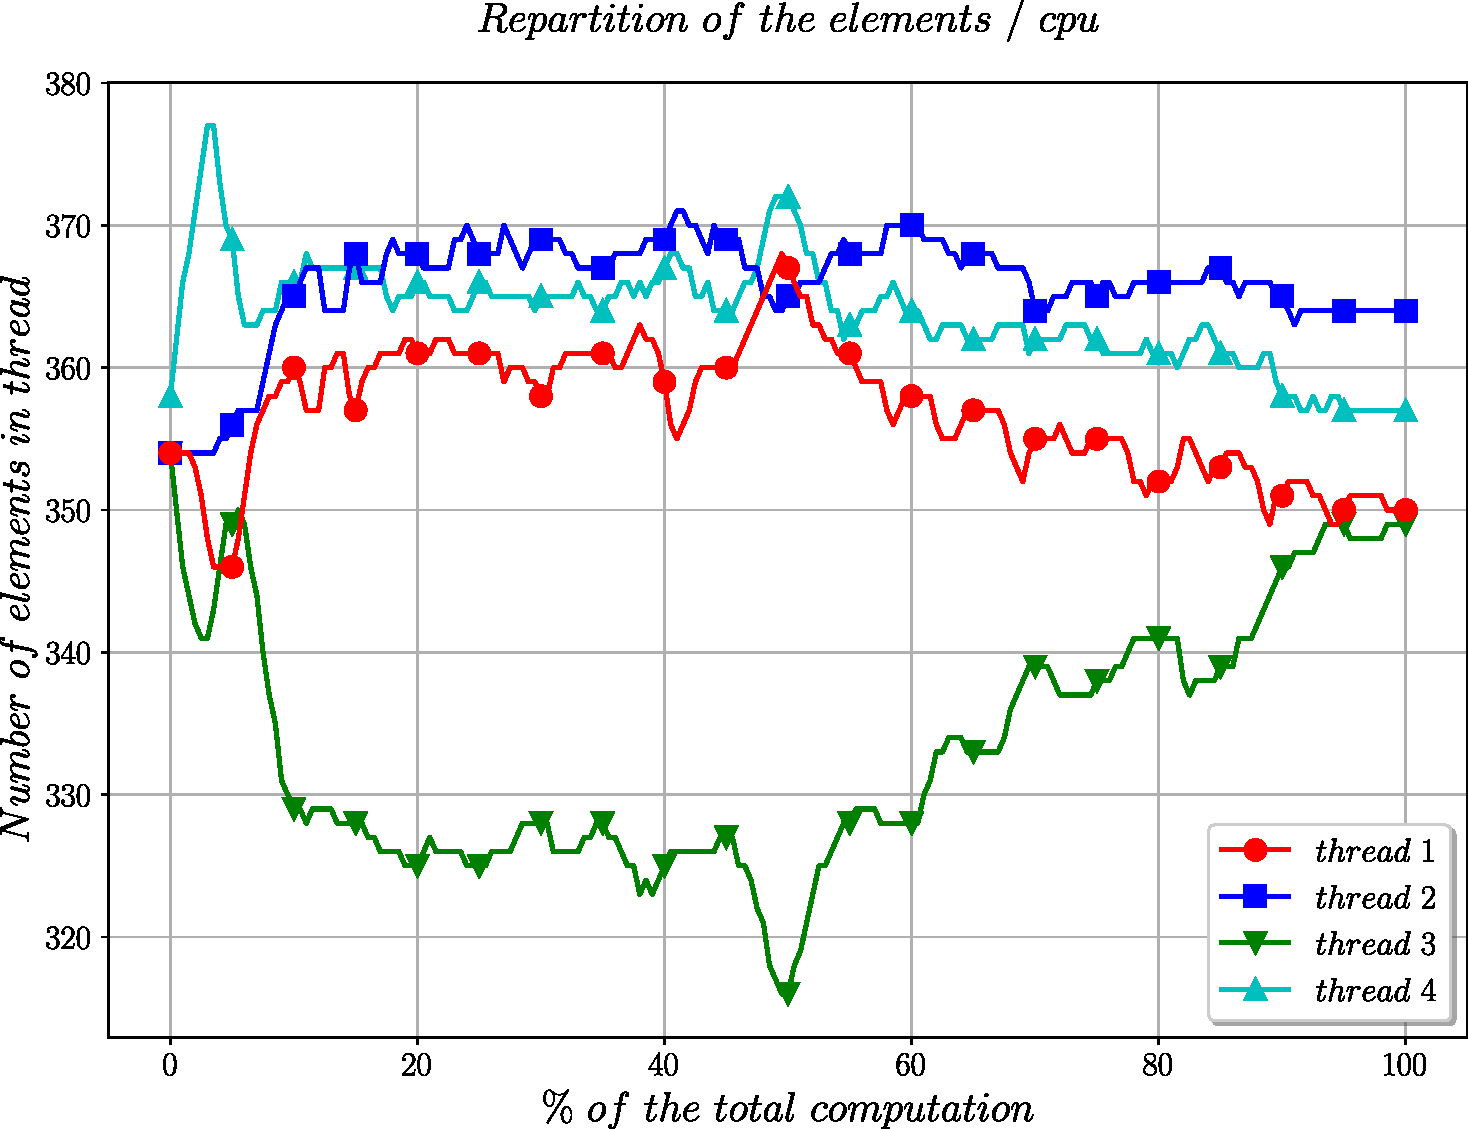
\includegraphics[width=0.75\textwidth]{./timethreads.pdf}
  \caption{Distribution of the elements during computation}
  \label{timethreads}
\end{figure}

\section {Conclusions}

In conclusion of this study, it was thus shown that 15 years after the publication of the original article \cite{Pantale:2005} concerning the parallelization of the DynELA Finite Element code, the results obtained previously are reproducible. It is still possible, with some adjustments to the margin, to recompile the code as proposed in 2005 (about 2 days of work were necessary to be able to complete the compilation of the DynELA code). The execution of the code on modern computing architectures does not seem to pose any problems, as no untimely crashes were noticed during the numerical simulations and the use of the code. The results in terms of performance with respect to code parallelization are in line with the results obtained 15 years ago, taking into account the radical change in hardware architecture for the execution of this Finite Element code.

In conclusion, we can also say that the work presented in the article \cite{Pantale:2005} is reproducible today. The future will tell us if in a few years, these results will still be reproducible on new hardware architectures.

